%%%%%%%%%%%%%%%%%%%%%%%%%%%%%%%%%%%%%%%%%
% Grant Template
% LaTeX Template
% Version 1.1 (26/12/19)
%
% This template originates from:
% http://www.LaTeXTemplates.com
%
% Original author:
% Erick Tatro (erickttr@gmail.com) with modifications by:
% Vel (vel@latextemplates.com)
%
% Adapted from:
% J. Hrabe (http://www.magalien.com/public/nih_grants_in_latex.html)
% By: Mackenzie Mathis
%
% License:
% CC BY-NC-SA 3.0 (http://creativecommons.org/licenses/by-nc-sa/3.0/)
%
%%%%%%%%%%%%%%%%%%%%%%%%%%%%%%%%%%%%%%%%%

%----------------------------------------------------------------------------------------
%	PACKAGES AND OTHER DOCUMENT CONFIGURATIONS
%----------------------------------------------------------------------------------------

\documentclass[11pt, notitlepage,a4]{article} % Default font size and suppress title page

\usepackage[utf8]{inputenc} % Required for inputting international characters
\usepackage[T1]{fontenc} % Output font encoding for international characters
\usepackage{palatino} % Palatino font
\linespread{1} % A little extra line spread is better for the Palatino font
%\usepackage{helvet} % Helvetica font
%\usepackage{newtxtext} % Time New Roman font
\renewcommand*\familydefault{\sfdefault} % Use the sans serif version of the font

\usepackage{amsfonts, amsmath, amsthm, amssymb} % For math fonts, symbols and environments

\newcommand\gsubaim[1]{\textbar~\textbf{#1}}
\newcommand\ganttaim[4]{%
    \ganttbar{#2 \gsubaim{#1}}{#3}{#4}%
    }


\usepackage{setspace}
\usepackage{epstopdf}
\usepackage{enumitem}
\usepackage{verbatim}
\usepackage{dblfloatfix}
\usepackage{algpseudocode}
\usepackage{amsmath, mathtools, amsfonts}

\usepackage{comment}

\usepackage{multirow}

%\usepackage[showframe]{geometry}
\usepackage{sidecap, caption}

\usepackage{booktabs,longtable}
\usepackage{subcaption}
\usepackage{graphicx}% Include figure files
\usepackage{dcolumn}% Align table columns on decimal point
\usepackage{bm}% bold math
\usepackage{graphicx} % Required for including images
\usepackage{hyperref}
\usepackage{booktabs} % Nice rules in tables
\usepackage{wrapfig} % Required for text to wrap around figures and tables
\usepackage[labelfont=bf]{caption} % Make figure numbering in captions bold
\usepackage{sidecap} 
\usepackage[top=0.6in,bottom=0.6in,left=0.6in,right=0.6in]{geometry} % Page margins

\usepackage[font=small,labelfont=bf]{caption}
\usepackage{xcolor}

\pagestyle{empty} % Suppress headers and footers

\newcommand\circled[1]{%
  \tikz[baseline=(X.base)] 
    \node (X) [draw, shape=circle, inner sep=-1, fill=black, text=white] {\strut \footnotesize #1};%
}
\usepackage{hyperref}
\hypersetup{
    colorlinks=true,
    linkcolor=black,
    filecolor=magenta,      
    urlcolor=blue,
}

\hyphenation{ionto-pho-re-tic iso-tro-pic fortran} % Specifies custom hyphenation points for words or words that shouldn't be hyphenated at all
\pagestyle{plain}

%-----------------------------------------------------------------------------------------
%INSTRUCTIONS

%This assignment aims to sharpen your scientific formulation skills as a systems neuroscientist. Writing a research proposal will help develop your ability to craft coherent research questions, design appropriate experiments, and anticipate potential outcomes. This exercise is also intended to enhance your critical thinking and scientific writing skills. There is no set topic, you are free to consider ideas or topics that are most interesting to you, but please consider a “systems neuroscience” approach to your question.

% Objectives:
% ● To formulate a clear and concise scientific hypothesis.
% ● To design a methodological approach using the tools of systems neuroscience for testing the hypothesis.
% ● To predict possible outcomes and their implications.

%Reminder: You are not allowed to use LLMs (ChatGPT) to generate or write this assignment. IF you want to use ChatGPT (or equivalent) for “fine-tuning” for grammar and clarity, you are allowed to do so, but you must declare this at the end of your document. You are fully responsible for the contents of this work. Please remember that plagiarism is a serious offense at EPFL.


%----------------------------------------------------------------------------------------

%----------------------------------------------------------------------------------------
\begin{document}

\onehalfspacing

\begin{titlepage}
    \newgeometry{left=3cm,bottom=0.1cm,top=2.5cm}
	\centering
	{\textbf{ECOLE POLYTECHNIQUE FEDERALE DE LAUSANNE}\par}
    \vspace{1 cm}
	
\includegraphics[scale=0.6]{figures/Logo_EPFL.pdf}\par\vspace{1cm}
Systems Neuroscience | NX-435\par
	\vspace{1cm}
	{\scshape\Large\textbf{A title}\par} % to complete
	\vspace{1 cm}

    Research proposal
    \vspace{0.5 cm}
    
	{\large\textbf{Your name}\par} % to complete
	
	\begin{flushleft}
	
	\vspace{5cm}
	
    \vspace{0.5 cm}
    \vspace{2 cm}
    
    \end{flushleft}
% Bottom of the page
	{\large \textbf{\textit{26$^{th}$ of May 2024}}\par}
\end{titlepage}


\setcounter{page}{1}
\begin{center}


\end{center}

%----------------------------------------------------------------------------------------


\section*{Summary}
\vspace{5pt}

max. 2 paragraphs
 Answer the  "what, why, and how" questions:\\
 - What are you doing?\\
- Why is it important to perform this work (motivations)?\\
 - How do you intend to make progress (what do you intend to do to contribute to the issue and/or improve on the start-of-the-art)\\

\textbf{Proposed structure:} You can have a first part (similar to an abstract) quickly summarizing the state of the art, and what you plan on doing. Then present your aims --- that you will expend in the research plan --- into one paragraph, with ~one sentence summarizing each of the Aims/Sub-Aims.



%---------------------------------------------------------------------------

\section{Background \& Introduction} 
% remove the below instructions in your final version:
1 page max

- Provide a brief overview of the field and related work to your idea.\\
- Define the problem your research aims to address.\\
- Discuss the relevance and importance of your proposed study.

%---------------------------------------------------------------------------
\section{Research Plan}
% remove the below instructions in your final version:
1-2 pages max

- This part should include the 2 following required sections, Aims and Methods.

\noindent (1) Scientific Aim(s) \& Methods:\\
Here, you should clearly state your \textbf{hypothesis} you intend to test.\\

% Proposed structure: You can for instance list the aims presented in your summary, and describe each one with a small overview of the aim, **where you clearly state the hypothesis** and a paragraph on expected outcomes and another one on pitfalls and alternative strategy:

- Methods: Outline the experimental design, key tools, and controls; i.e., if you plan to write about designing a study that uses optogenetics, define which opsin, cite the relevant paper, and describe the design of the experiment. Or, if you want to design a new task-driven model of say, olfaction, which model architecture do you choose and why, etc.\\

\noindent (2) Anticipated Results:\\
- Discuss the expected outcomes of your experiments.\\
- Alternatives: What could go wrong and how can you mitigate them? (what if the mice don’t learn the task? Do you have a ``back up plan"?)\\
- Broader Impact: How will your study advance the field? Are their ethical considerations?

% here is an example figure input:
\begin{figure*}[ht] 
\centering 
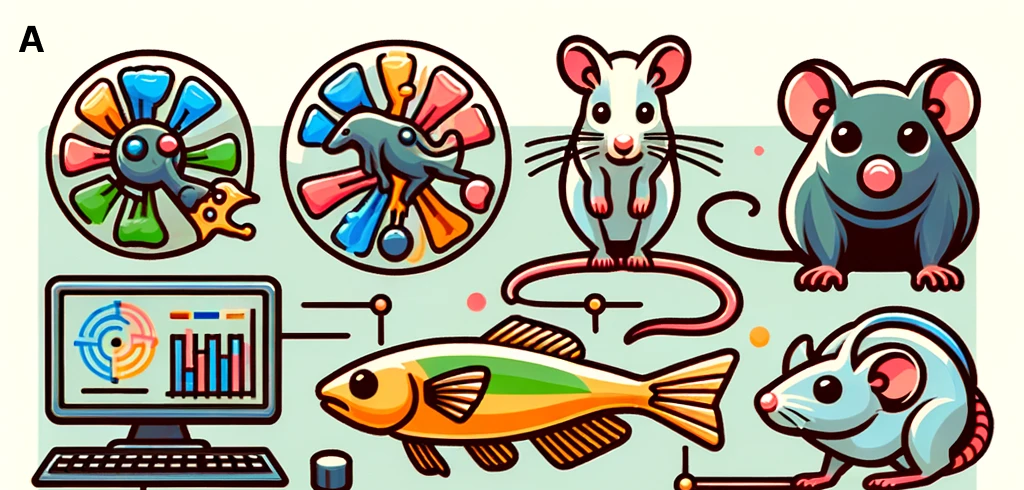
\includegraphics[width=.5\textwidth]{figures/figure1.png} \caption{\textbf{My Cool Figure.} 
\textbf{a:} A whimsical view of systems neuroscience, courtesy of prompting by M. Mathis to GPT-4/DALLE.
}
\label{fig:Figure1} 
\end{figure*}

%---------------------------------------------------------------------------
\section{References}
\bibliography{references}


%----------------------------------------------------------------------------------------

\end{document}